\documentclass[acmsmall,screen,nonacm]{acmart}

% ACM class controls page geometry, typography, headings, and float styling.
% Do not add geometry or manual spacing overrides.
\usepackage{microtype}
\usepackage{xurl}

\setcopyright{none}
\settopmatter{printacmref=false, printccs=true, printfolios=true}

\title[Citation-Support Scoring Policies]{Citation-Support Scoring Policies Change System Gaps: A Controlled Reanalysis of Archived Human Annotations}

\author{Gorla Nitheesh Kumar}
\affiliation{%
  \department{Department of Information Technology}
  \institution{Indian Institute of Information Technology Allahabad}
  \city{Prayagraj}
  \state{Uttar Pradesh}
  \country{India}
}

\renewcommand{\shortauthors}{Kumar}

\begin{CCSXML}
<ccs2012>
 <concept>
  <concept_id>10010147.10010257</concept_id>
  <concept_desc>Computing methodologies~Natural language processing</concept_desc>
  <concept_significance>500</concept_significance>
 </concept>
 <concept>
  <concept_id>10002951.10003317</concept_id>
  <concept_desc>Information systems~Information retrieval</concept_desc>
  <concept_significance>300</concept_significance>
 </concept>
 <concept>
  <concept_id>10010147.10010257.10010293</concept_id>
  <concept_desc>Computing methodologies~Evaluation methodologies</concept_desc>
  <concept_significance>300</concept_significance>
 </concept>
</ccs2012>
\end{CCSXML}

\ccsdesc[500]{Computing methodologies~Natural language processing}
\ccsdesc[300]{Information systems~Information retrieval}
\ccsdesc[300]{Computing methodologies~Evaluation methodologies}

\begin{document}
\begin{abstract}
Comparisons that rely on citations (evidence) rely on the credit given to partial supporting sources. In this work, such dependence is explored with the set of answers fixed in the archives and human annotations from Liu et al. We employ a conditional-credit control (C0) and an individual-full-support-only control (C1). It is not possible to have the same original evaluation due to the archive not defining all the conventions for counting occurrences, repeated records and aggregation. For this reason we employ a separately specified, auditable adaptation: unique raw response records, one-to-one occurrence–judgment links, positive citation denominators and equal query weights on a four-system common cohort. The experiment is to be performed with 353 queries. While Bing Chat, Neeva, Perplexity and You are 0.826, 2.111, 3.753 and 1.220 percentage points less precise on average, respectively. The greatest pairwise difference in change is 2.927 points, and there is no change in ties or order in the six system pairs. Loss is focussed in a minority of responses. Ordering is preserved in the tested conditions in alternative duplicate handling and pooled-citation aggregation. These are descriptive results with regard to an historical archive, not product rank results, a verified original-cohort reproduction, and/or a claim of methodological novelty.
\end{abstract}
\keywords{citation support, scoring sensitivity, reproducibility, human annotations, generative search}
\maketitle

\section{Introduction}
Even a real source can be cited and not support the statement that it is cited to!A citation can refer to a real source and not support the statement cited to it~\cite{liu2023,rashkin2023}. This distinction was enough to inspire our previous literature review on fabrication of citations, misattribution and corruption of metadata. The present implementation commits to a very broad review but restricts it to one quantifiable issue: what happens to comparisons when the answers and the human judgments are constant. Doesn't validate bibliographic accuracy or return webpages or provide new answers.

Evidence can also be disseminated. If a sentence states two propositions and different sources backup different propositions, then the combination of the two sources may be sufficient to support the two together even if neither source is sufficient on its own. On the other hand, an irrelevant citation can be supported by a "supporting source. In order to be useful, a protocol must thus distinguish between the support of a statement by an evidence set and the credit of each cited member. This distinction is already reflected in the evaluation of citation generation~\cite{gao2023}; the open question is what are the numerical implications of these distinctions under one particular annotated archive?

This distinction is important when one reads back about performance. A precision gap is generally assumed as the degree of difference between systems while a ranking only keeps the sign. If a score change occurs, the order could remain the same but the size of the score change would be different. When looking at all pairs, one also won't focus on comparison that changes most, since the one that changes the least may be the most important. In the present design, the query distribution is the same for all systems, and the changes that are made are only partial-support credit in the primary comparison. It thus helps to identify the measurement effect from any improvement or deterioration of the generated content.

The verifiability study, initially developed by Liu et al., offers a helpful starting point for a methodology on verifiability~\cite{liu2023}. In addition, its precision rule acknowledges an important aspect of the contribution of partial sources: Several citations may contribute to a statement even if no single citation does so entirely. The elimination of this credit alters the meaning of precision as an operation. Does not have to be the same amount in each system. A change in the difference between systems is thus more informative than a system level reduction.

This paper contains a bounded computational question. How do the pairwise gaps change if the credit policy is altered but the observations, the units and the weights remain unchanged? This still yields meaningful results even when there is no ordering change. Rank stability and gap stability are not the same: the same order may occur with substantial differences in numerical gaps. On the other hand, a low mechanical score does not necessarily indicate a research contribution.

The first one was the original baseline B0 with the strict comparator B1. A lack of operational information was identified during the inspection. We don't adopt an undocumented convention that looks like published aggregate results, we preserve that limitation. These are henceforth referred to as our executed controls C0 and C1. C0 provides a new and explicit cohort and counting protocol to implement the published conditional-credit logic. This does not claim to be a full evaluation of the original paper.

This course level study includes (i) repeatable rational scoring with auditable mappings, (ii) pairwise gap sensitivity and concentration level at the response level, and (iii) duplicate handling, aggregation and failure analysis. There is no information available on the novelty of this exact reanalysis. There is no new algorithm, model or annotation data set claimed.

\section{Related Work}
\subsection{Citation-supported generation and verifiability}
Citation-supported generation is a relationship between an answer and an inspectable evidence, but the process of creating a relationship and supporting it is distinct processes. Liu et al.~\cite{liu2023} quantify this difference in terms of human evaluations of statement coverage and citation support. Their conditional precision rule gives a partial source only in a statement that is supported by a full source, other than an individually full source. In the present study, the logical predicate remains while the operational protocol for applying it to the archive is explicitly changed.

ALCE is designed to measure end-to-end retrieval and cited-answer generation, distinguishing between fluency and correctness of the answers and the quality of the citations~\cite{gao2023}. It applies natural language inference to evaluating citations and checks if a citation agrees with a statement or provides evidence for a statement in a supporting set of citations. Thus, citation precision is not merely the rate of citations that are present but not precise. Nor is ALCE's automated test, interchangeable with Liu's archived "human" categories. The support judgment, its granularity and the rule that is used to turn the judgment into credit are all methodological decisions.

These strategies also decouple the assessment from the generation. If the question stimulus (prompt/retriever) is changed, the answers being assessed will change, and if the credit rule is changed, the same answers will be assessed for a different credit. In our experiment, we separate out the latter operation. It can neither compare retrieval architectures nor suggest a strategy for the generation, but it can illustrate the extent to which a historical comparison depends upon what an evaluator will reward.

\subsection{Attribution and human support judgments}
The Attributable to Identified Sources framework is a formal mechanism for attributing to supplied evidence, while allowing for the context in which it is interpreted.The Attributable to Identified Sources framework is a formal way to attribute to supplied evidence that accounts for the context in which it is interpreted. It separates the actions of interpreting from assessing the evidence of whether or not the evidence supports. This is relevant for annotations that have been stored: a label is based on the statement, the source material and the instructions provided to the annotator, but not on a general assessment of truth. Also a statement level support label does not automatically indicate which specific source offers full support.

BEGIN assesses attribution in knowledge-grounded dialogue with human annotations, and identifies automated metrics that probe for errors related to abstraction and evidence length~\cite{begin}. The categories in its response level are to a different unit within a search answer to a cited marker. The comparison is used as a motivator to keep units and not all attribution scores equal. In this place, a statement may have multiple citation units with multiple judgements for each unit, and a collective judgement for the evidence.

There is a need for reliability evidence for human judgments. Artstein and Poesio~\cite{agreement} describe the differences in agreement measures based on the assumptions of coders, categories and chance agreement. The repeated rows can not be taken for granted as being independent raters or fresh answers. Inter-annotator agreement is not computed for repeated records that are not identified. Howcroft et al.~\cite{howcroft} record variation in human-evaluation terminology and reporting, further highlighting the importance of specifying the property to be evaluated and how this is done. Our raw labels and explicit normalization record is for that particular reporting purpose only, and not for the purpose of asserting the validity of the annotation itself.

\subsection{Factuality, groundedness and evaluation units}
Studies on summarization provide a rationale for separating support from a document from support for a document's truth. Maynez et al.~\cite{mayenz} study faithfulness and factuality with human assessment of hallucinations. Instead, FActScore breaks down long-form outputs into atomic facts and measures what proportion can be covered by a knowledge source~\cite{factscore}. It's atomic information, our's is mapped citations within responses. Neither the resulting percentages nor changes in them are directly comparable. We don't add atomic decomposition after the archived statements.

There are still other operational routes that can be illustrated using automated consistency methods. For the consistency judgments, FactCC learns them from transformed source sentences, it also contains evidence-span extraction~\cite{factcc}. QAGS does comparisons among answers to questions on the summary and source~\cite{qags}. QAFactEval explores the impact that question construction and the question answerability properties of the components have on QA-based consistency assessment~\cite{qafacteval}. These techniques are used to make predictions about semantic judgments; our controls use already made judgments. To introduce a second annotator would introduce prediction error and change the experimental question.

Even if only a single final score is reported, granularity and error type are important. SummaC tackles an issue where there is a mismatch between the inference from a particular sentence and the overall consistency of the document, aggregating sentence-pair evidence~\cite{summac}. FRANK offers a taxonomy of factual errors and examines the strengths of the metrics for each category of error~\cite{frank}. These studies call our attention to units and failure modes, but do not support our citation-occurrence mapping. This check is performed directly with the archive. Likewise, a syntactically ambiguous marker is not necessarily a semantic hallucination.

RAG evaluation broadens the set of relevant constructs. Automated assessment~\cite{ragas} is used by RAGAs to separate context retrieved features from answer relevance and faithfulness. ARES trains evaluation judges and merges their predictions with human annotations by prediction-powered inference~\cite{ares}. RAGTruth also provides spans that are manually labelled with hallucinations for retrieval-augmented outputs~\cite{ragtruth}. All differentiate between evidence-conditioned output quality and simply having the retrieved text. Their procedures to make a prediction, train and uncertainty, however, are not a part of this experiment. There is no model judge added to this finite-archive analysis, nor does it benefit from any confidence guarantees from other models.

\subsection{Measurement sensitivity and reproducibility}
Validation for metrics should be done to distinguish between agreement at the system level and agreement on individual examples. SummEval not only includes system-level correlations, but also explicitly seeks to evaluate the examples at a higher level than that provided by an expert or a crowd in the common summarization evaluation~\cite{summeval}. This distinction is also used to report average losses as well as their distribution by response level. Comparing the behaviour of two policies on the same answers is not possible based on stable ordering alone.

Another question is, does a score define its computation sufficiently? This is illustrated in post~\cite{post} by showing that BLEU reporting can mask significant differences in preprocessing and/or parameters. That outcome is not about the accuracy of the translation, but it is about the principle of reporting, not a transferred effect size; this is why it is pertinent here. Weights and eligible records, like weights without a denominator, also do not fully specify our measurement. The sensitivity analysis therefore decomposes changing citations into the change in citation credit and the change in aggregation.

Belz et al.~\cite{belz} examine challenges in repeating the human evaluations and reproducing the results. Their conclusions lead to a delicate balance between reuse of released judgments and re-constructing an original study. Data statements also help document the composition of the data and appropriate generalization~ \cite {datastatements}. The selected cohort can be inspected in our archive identity, exclusion audit and source coverage records, but cannot be reconstructed from undocumented original decisions and will not be representative of a restricted cohort.

\subsection{Position of this study}
Previous studies define attribution frameworks, human support evaluation benchmarks and automated factuality benchmarks. It examines a narrower question, that of how a declared change in the credit-policy affects six pairwise system gaps, given that judgments and eligible responses are assumed to be archived and therefore remain constant. It does not propose a new support concept, a new metric predictor or a complete reliability benchmark, it's just an auditable local comparison. The increased literature provides context, but not the novelty of this particular comparison.

Liu, ALCE, FActScore and RAGTruth were already recognized in the previous review. The rest of the scholarly writings are methodological contextualization, which is documented in the reference-verification files. The partially identified study of Zhang is not included. The original review has not been altered and the bibliography remains the same.

\section{Research Questions and Study Positioning}

\textbf{RQ1 (supporting):} Where does the policy sensitivity lie for each system on the fixed eligible cohort? \textbf{RQ2 (primary):} How does the policy change affect each of the pairwise system precision gaps? \textbf{RQ3 (supporting):} Does it affect relative ordering, including exact ties and strict reversals?

There is no need for an empirical hypothesis to be directionally formulated. It turns out that, for the fixed positive denominators and non-negative weights, it is mathematically required that C1 must be less than or equal to C0. The degree of differences in losses from system to system, the degree of change of the gaps, and the sign change of the gap are empirical questions. For each of the six unordered pairs, we give them in the order Bing Chat, Neeva, Perplexity, You. We don't set a practical-effect threshold based on the results. The significance of the findings is left to the reader given that the findings are reported as percentage points.

\section{Data and Reproduction Boundary}
\subsection{Archive identity and structure}
The data is read from the authors' companion repository (commit \texttt{2c6b485ae1c2} of the configuration file): \texttt{human\_evaluation\_annotations.jsonl} The file size is 17,520,509 bytes and the validation report of the repository contains the SHA256. All records are JSON objects. The validation independently counts 5,528 annotation rows, 5,457 distinct response IDs and 1,450 exact query strings. These names are not to be confused with the current service configuration names. There are four historical systems.

The query, response, system, source category and citation objects with character offsets, plus the mappings from statement to marker and the nested human judgments are stored in a record. Original strings and labels retained. The raw JSONL record is identified by a technical line index. The following rows are output rows that are associated with that index, response ID, statement ordinal, judgment ordinal, and citation-object index. This gives the ability to trace each credited unit without sharing the text of responses or selected source text with other units.

\begin{table}[t]
\centering\small
\caption{Independently checked archive structure. Counts precede exclusions.}
\begin{tabular}{lr}\toprule
Quantity & Count\\\midrule
Annotation rows & 5,528\\
Distinct response IDs & 5,457\\
Repeated-ID groups & 69\\
Excess structurally identical records & 47\\
Repeated groups with distinct records & 24\\
Citation objects & 15,828\\
Statement--marker entries & 15,169\\
Rows with unequal object/entry counts & 335\\
Zero-citation rows & 892\\
Null collective judgments & 9,075\\\bottomrule
\end{tabular}
\label{tab:structure}
\end{table}

\subsection{What the original baseline does not establish}
The formula used to calculate the response level of the paper is
\begin{equation}
 P_0=(T_{fs}+T_{ps})/N_{\mathrm{paper}}.
\end{equation}
The denominator is referred to as the total citations in a response. There are various ways of displaying citations in the archive. There are 335 rows in which citation-object counts and statement--marker counts have different values. There can be several markers in one statement that have the same associated judgement for that statement. The following formula is not correct: one judgement in the numerator and all the occurrences in the denominator, since the propagation convention has to be specified.

If an ID is repeated for a response, the policy needs to be repeated. Records in the archive are structurally similar and also have different annotations for an identical response. The original selection/combination convention was not restored. Taking the first row; or averaging distinct records is not evidence of what the original authors did. The ratio only allows for a definition of zero-citation precision, and the original treatment in aggregation has not yet been precisely determined. The repository inspected was not able to provide the correct original precision-scoring script.

Thus, DEN-01, DUP-01 and AGG-01 will continue to be open to original cohort replications. No published aggregate values are used to guide our decisions of processors. We make no numerical replication claim. This is validating the behaviour of the adapted controls, under the contracts they claim.

\subsection{A conservative operational adaptation}
We had a protocol configuration saved ahead of time stating the following main rules. First, if the records in the response are all structurally the same, yet the response ID is repeated, exclude all such repetitions. Second, ensure there is a unique row in the raw data for each query and system. Third, confirm each citation object's half-open character span for each response text that is not altered. Fourth, find every exact sub-string of that response that corresponds each to one of the cited statements. There must be exactly one judgment for each statement-marker, and there must be exactly one citation object for each of those judgments, and all of the citation objects must be used exactly once. Equality of count alone is not enough.

If the response contains ambiguous information, a missing required judgment, or an unfamiliar label or a mapping that does not match, the response is ineligible for both controls. Positive citations must be provided. Lastly, cross-intersect qualifying exact query strings within all four systems. There are 353 queries, 1,412 responses and 4,382 mapped citation units in the primary intersection. The previous 357-query structural screen was not the last group: The more robust bridge validation also verifies actual correspondence. There is no text normalization or paraphrase merge of query text.

This restriction narrows a set of questions the answers to which are known to be cited in some way by every system. It cannot make claims on answers which do not appear in its answer, or for missing answers, or for the entire distribution of the archived query. There are 12 categories, and these are the same as in the raw source coverage table, but all categories have been weighted differently. The above is intentional as no model fitting, threshold optimization or learned parameter selection are done.

\section{Scoring, Estimands and Implementation}
\subsection{Adapted controls}
Let $N_r$ be the number of objects $r$ that are cited bijectively. This is an operational denominator for this adaptation, not a solution of $N_{\mathrm{paper}}$. Count the units in $F_r$ by single units. Each statement only contributes to $H_r$ if its collective judgment is Yes, but at least one individual judgment is not full. The two controls are the ones of our own.
\begin{equation}
 C0_r=\frac{F_r+H_r}{N_r},\qquad C1_r=\frac{F_r}{N_r}.
\end{equation}
Partial units are otherwise not added to the numerator and do not earn any credit. A fully earned citation will not deduct conditional partial credit for the other citations on the same statement; it only will suppress them from the denominator.

The documented exceptional individual labels of the repository are mapped to “no support”: inaccessible, unclear, support plus refutation. Normalized classes are kept with raw labels next to them. Partial credit is not allowed for collective No judgment or conflicting-citation judgments. The inspected archive has 9,075 collective judgments that are null, which are not related to any mapped citation. Evidence excerpts that are blank do not affect the support decision. Our scorer does not give in to unanswered questions, he does not guess the class.

Two part statement, two partial sources and collective full support is C0=1, C1=0. If there is a full source, plus a partial source, then both the full source and the partial source have the C0 value of 1/2. They are not measured archive outcomes but cases hand-created for validation. They explain that conditional partial credit and half-credit are different rules.

\subsection{Pairwise estimand}
For the common query set $Q$, each system has one retained response per query. Define
\begin{align}
 P_{s,k}&=|Q|^{-1}\sum_{q\in Q} Ck_{s,q},\\
 L_s&=P_{s,0}-P_{s,1},\\
 G_{ab,k}&=P_{a,k}-P_{b,k},\\
 D_{ab}&=G_{ab,1}-G_{ab,0}=L_b-L_a.
\end{align}
The final result is the 6-component vector $D$. The signed advantage of a over b is increasing as a result of strict scoring if positive Dab. It does not necessarily indicate that either system gave a better answer. Precision is a measure that supports and loss/gap sensitivity are descriptive quantities that do not have an inherent direction for optimization.

The loss at response level is $H_r/N_r$. From $N_r>0$ and $H_r\geq0$ it is immediately seen that $C1_r\leq C0_r$ without making any empirical assumption. At the system level, $L_s$ is the average of these fractions with no division of the pooled partial count by a pooled denominator. In the aggregation sensitivity analysis, the latter is a citation weighted average, where the weight of the response $r$ is $N_r/\sum_{r'}N_{r'}$. The two weighting schemes are designed to answer two different types of questions, the query and the typical citation, respectively.

All comparisons are with exact rational arithmetic. Strict reversal means that the two gaps must have opposite nonzero signs. A tie transition is when equality is met to exactly one policy. Rounded display values never determine these categories. No significance test or confidence interval is added: the goal is not to give an interval or test for this limited sample of the selected archive annotated by inheritance, but a sampled population of new model generations. Citations within a response, repeated annotation records and answers to the same query are dependent observations.

\section{Experimental Design and Validation}
The implementation is based on the standard libraries of Python. Record loading and validation, reconciliation of annotations, cohort construction, scoring of each control and aggregation of metrics are all performed via separate modules. Functions throw errors if the denominator is zero or is different from the other denominator. The original B0 entrypoint throws unimplemented-method explicitly, thereby avoiding the confusion of an adapted implementation being regarded as a faithful implementation.

There are 18 unit tests that include full, partial, judgment that is unsupported or judgment that is contradictory, conditional suppression, nulls, zero denominators, repeated markers, wrong offsets, repeated IDs, and invalid JSONL. Individual examples are complemented by exhaustively considered small-label configurations. An independent arithmetic audit does not import the scorer, reads raw labels, re-computes response fractions, aggregates and checks all exact system scores and pairwise gaps in all three cohort variants. It verifies 4,346 scored record cases for those variants. This is not a human assessment of the source support independent of arithmetic.

This session tried to access the path of the user's laptop, which is reported to be a WSL2/i3 environment. The executed evidence was created from the assistant's Linux workspace using Python 3.12.14. The code has been written with features of the standard library that are compatible with Python 3.11 and the end pipeline has not been executed again on the user's Python 3.11.18 environment. Figures were created using matplotlib 3.10.8. No model, GPU, training or paid API involved. That workspace had a clean run time of 9.755 seconds including the tests, validation, analyses, audit and figures; max child resident set size was 87,524 KiB. This is not a laptop benchmark, just a measure of this run.

\section{Results}
\subsection{System losses and concentration: RQ1}
The results for 353 common queries are shown in Table~\ref{tab:system}. Perplexity has the largest mean loss (3.753 points), followed by Neeva (2.111), You (1.220) and Bing Chat (0.826). The median response loss is 0 for each system. The affected-query counts are 4, 16, 27 and 6 respectively in the table's system order; these correspond to 1.13\%, 4.53\%, 7.65\% and 1.70\%. Thus, on the aggregate, an affected subset of small size represents each policy difference.

\begin{table}[t]
\centering\small
\caption{Primary results. Precision in percent; loss in percentage points. Affected counts are out of 353 queries per system.}
\begin{tabular}{lrrrr}\toprule
System & C0 & C1 & Loss & Affected\\\midrule
Bing Chat & 91.792 & 90.966 & 0.826 & 4 \\
Neeva & 69.187 & 67.076 & 2.111 & 16 \\
Perplexity & 76.295 & 72.542 & 3.753 & 27 \\
You & 62.367 & 61.147 & 1.220 & 6 \\
\bottomrule

\end{tabular}\label{tab:system}
\end{table}

\begin{figure}[t]\centering
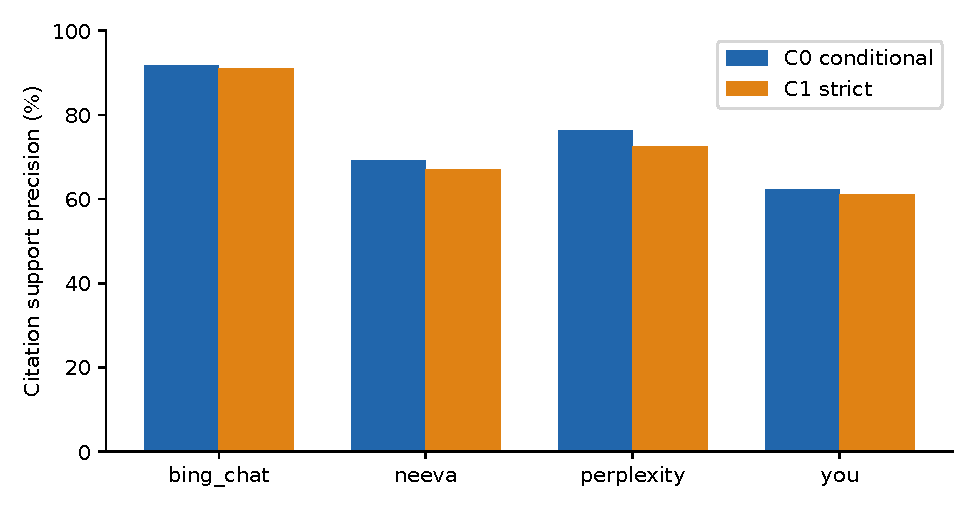
\includegraphics[width=\linewidth]{figures/precision.pdf}
\caption{Shared-cohort precision under both adapted controls. The chart starts at zero; differences are detailed in Table~\ref{tab:system}.}\Description{Grouped bar chart comparing C0 and C1 citation-support precision for Bing Chat, Neeva, Perplexity, and You. C1 is lower for all four systems.}\label{fig:precision}
\end{figure}

Each system loses a max of 100 points. That can be done if none of the credited citations provides a full support for a particular statement in the context of partial credit for all of the statements. It isn't evidence the answer changed from true to false as a result of the new policy. The empirical cumulative distribution is thus highly peaked at zero and has a small tail. Reporting just an average would conceal this concentration and reporting only the extreme cases would inflate the prevalence.

\subsection{Between-system gaps: RQ2}
The table below shows all six comparisons, but no selection based on the result of the comparisons.All six comparisons are listed in table~\ref{tab:gaps} without making any selection based on the outcome of the comparisons. The biggest difference is between Bing Chat and Perplexity, which goes from 15.497 to 18.424 points, a margin of 2.927 points. The Perplexity--You gap decreases by 2.533 points, from 13.928 to 11.395. These changes are not due to different answers nor annotations.

\begin{table}[t]\centering\scriptsize
\caption{Pairwise gaps and changes, all in percentage points. Pair orientation is fixed before scoring.}
\begin{tabular}{lrrr}\toprule
Pair ($a-b$) & $G_0$ & $G_1$ & $D$\\\midrule
Bing Chat--Neeva & 22.605 & 23.890 & +1.285 \\
Bing Chat--Perplexity & 15.497 & 18.424 & +2.927 \\
Bing Chat--You & 29.425 & 29.818 & +0.393 \\
Neeva--Perplexity & -7.108 & -5.466 & +1.642 \\
Neeva--You & 6.820 & 5.928 & -0.891 \\
Perplexity--You & 13.928 & 11.395 & -2.533 \\
\bottomrule

\end{tabular}\label{tab:gaps}
\end{table}

\begin{figure}[t]\centering
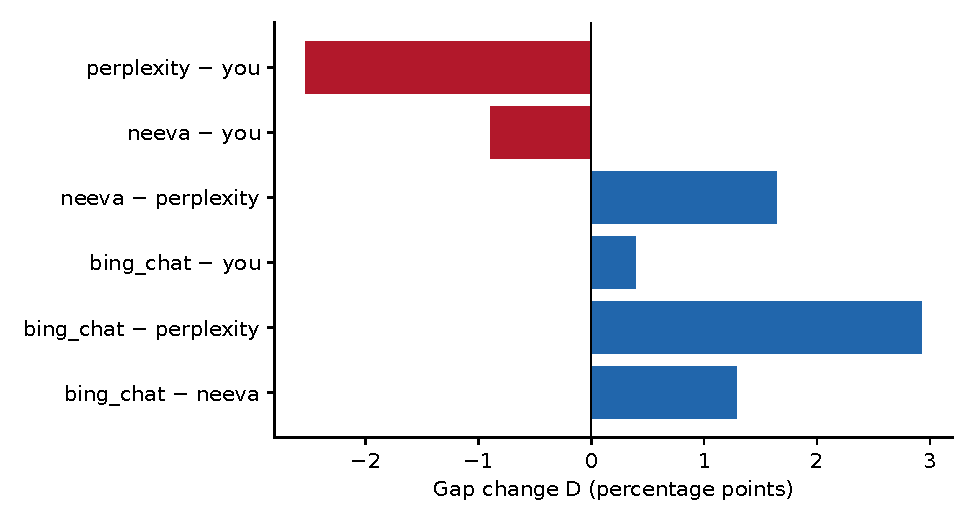
\includegraphics[width=\linewidth]{figures/gap_changes.pdf}
\caption{Primary gap changes. Positive values increase the signed advantage of the first system; negative values decrease it.}\Description{Horizontal bar chart showing six pairwise precision-gap changes. Three changes are positive and three are negative; the largest absolute change is 2.927 percentage points for Bing Chat versus Perplexity.}\label{fig:gaps}
\end{figure}

The identity Dab=Lb-La is verified precisely by the implementation and independent audit. For its scientific application, it is explanatory, meaning that all of the change in separation is due to the varying conditional partial credit in the fixed cohort. It does not provide any rationale for the generation of the citation patterns in historical systems. In this analysis, the details of prompt and retrieval behavior and the model architecture were not manipulated or measured.

\subsection{Ordering: RQ3}
Both policies instruct the previously retained historical systems as Bing Chat, Perplexity, Neeva and You. No two comparisons in the six pairwise comparisons are exactly tied or have a tie transition or strict reversal. This is a negative result in ordering instability under this adaptation. It doesn't mean that scoring choice is not important; the differences in scores do change. Also, it doesn't support rank stability under other cohorts, source distributions, annotation conventions or current product configurations.

\section{Sensitivity and Robustness Analysis}
\subsection{Repeated-record decisions}
The two declared alternatives are repeated-record treatment. The first removes all the same records and leaves out groups of records. The second stores one of each of the structurally different records and then averages the scores of each of these records in a response/query. This is clearly an average of archive data and not an average over hypothetical annotators. All of these still need to have an occurrence bridge and all system query coverage.

The alternatives keep 363 and 369 queries, respectively; see Table \ref{tab:robustness}. There is no change in the order of the items in either. Based on the primary analysis, the Bing Chat--Perplexity gap change is 3.066 and 3.125 points, respectively, while for the Bing Chat it is 2.927. These differences include record-resolution and cohort-expansion effects. Do not consider them as an unqualified cause/effect assessment of duplicate handling. For the unchanged primary cohort, there are no additional records to average for the repeated-record alternatives, and the only meaningful comparison is with the sensitivity of the overall eligible-archive analysis to those policies.

\begin{table*}[t]\centering\small
\caption{Duplicate-handling sensitivity. System columns report mean precision loss in percentage points. Cohorts differ; this is not an isolated fixed-cohort annotation effect.}
\begin{tabular}{lrrrrr}\toprule
Variant & Queries & Bing Chat & Neeva & Perplexity & You\\\midrule
Primary & 353 & 0.826 & 2.111 & 3.753 & 1.220 \\
Identical collapse & 363 & 0.803 & 2.466 & 3.870 & 1.462 \\
Distinct mean & 369 & 0.790 & 2.426 & 3.915 & 1.573 \\
\bottomrule

\end{tabular}\label{tab:robustness}
\end{table*}

\subsection{Aggregation sensitivity on the same cohort}
A second analysis pools citation counts within each system instead of equally weighting responses. It takes the same main observations and unit denominators, but changes the weights of aggregation: answers with a higher number of citations have more influence. This is not a correction for the main result, but a separate estimand that is not related to the main aggregation convention of the original result.

If it is aggregated in the pooled manner, the difference in change between Bing Chat and Perplexity is 2.996 points, while the difference in change between Perplexity and You is $-1.872$ points. The order of all pairs is again the same. The difference from the macro analysis is that the two types of citation-credit policy and aggregation contribute to the difference in numbers. We don't select the one that makes the greatest difference as the primary outcome.

\begin{figure}[t]\centering
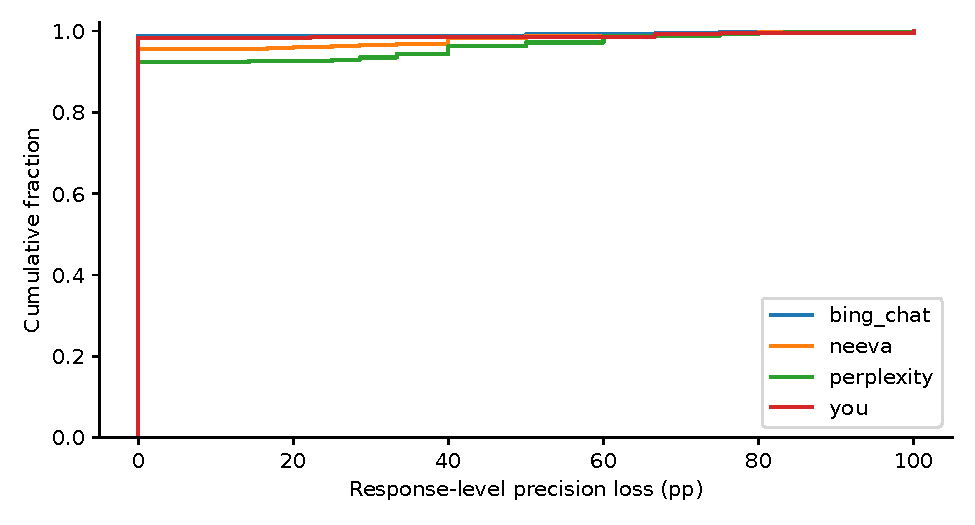
\includegraphics[width=\linewidth]{figures/loss_ecdf.pdf}
\caption{Response-level loss distribution. All four medians are zero; positive loss is confined to a small subset.}\Description{Empirical cumulative distribution curves for response-level precision loss across Bing Chat, Neeva, Perplexity, and You. All curves show a median loss of zero and a small tail of positive losses.}\label{fig:lossdist}
\end{figure}

\section{Failure-Case Analysis}
The 345 rows flagged by the mapping audit have a non-bijective marker-to-occurrence correspondence, the 335 rows flagged by the mapping audit have different object and unit counts, and the 12 rows flagged by the mapping audit have nonunique or non-existent exact span of statements for the statement. These are not categories of addition. The 892 zero-citation rows are kept in the audit but do not have precision and are not entered into the primary cohort. These rows would not be automatically abstentions and giving them a score of zero would address a different question.

In the raw distribution of labels there are 324 labels that cannot be accessed, 139 are support-plus-refutation and 33 are unclear in the complete archive. Their normalization is zero credit, and their interpretations continue to be different from the documented categories. Not accessible means not absent; not clear means not false. Even with the support-credit behaviour fixed, these cases are helpful in identifying the cases of construct confusion.

The failure case table contains raw line/response ID instead of publishing of excerpts. A reviewer with verified archive can review the statement and offsets. If an ambiguous response is not included, it means that the entire query it represented is excluded from the all-system cohort, and can take the other systems' otherwise usable answers out of play. This is the cost for comparability, and results in a significant amount of selection bias.

\section{Discussion}
Observed result distinguishes three propositions. First, no contract can improve precision under the fixed contracts, as is evident from the formula. Secondly, different systems lose different amounts of credit, so that pairwise gaps move; this is measured. Third, the gaps tested do not intersect zero; in this case ordering is stable. The latter two are the observed archives. Mixing them up would result in a mathematical invariant being put to the test as an empirical finding or mask a negative ordering result.

The strict policy should not be automatically assumed to be more accurate. A citation may be useful for providing partial legitimate evidence in a statement that is supported by the group. C0 rewards that contribution; C1 asks whether each cited source is sufficient on its own. But which construct should be used depends upon the purpose of evaluation. C1 might be a better option for a reader who must take the whole block of support from each of the links or C0 might be a better option for an evaluator who believes that the evidence synthesis is more important. Our experiment does not aim to decide which of the two choices is better or worse in all circumstances; it only documents the results of our particular choice.

Also, the concentration result is relevant when considering an average gap. This policy change has no impact on the majority of retained responses. A small percentage of these can still cause a change in system separation, as a response level average assigns equal weight to every query, including short responses with a high conditional-credit component. The pooled-citation analysis adjusts this weighting and so does not necessarily result in the same gap changes. Both analyses do not provide any indication of the value to users of answers or the seriousness of any unsupported claims.

There is no way to resolve what this result doesn't resolve, unless you do a literature comparison. An attribution framework provides evidence relations and an automated factuality benchmark measures the ability of a predictor to recognize evidence relations. Rather than that, we test a deterministic transformation of inherited labels in our study. Arithmetic validation will not prove those labels to be correct, and a non-changing system order will not prove an automated judge. These are distinct evidences required.

An important reporting implication in practice is to include a counting unit for a precision value, along with a rule for eligibility and partial credit and aggregation weights. The reporting of both policy losses and of collective change events reveals if a comparison is bias because of unequal credit for collective support. This is a recommendation based on the observed sensitivity, rather than an assertion that the recommended policies are the only reasonable evaluation options. If a wider comparison were used, more annotated evidence of the independence of the comparison would be required and more definitions should be justified.

The restrictive cohort is a good aspect and a disadvantage. It eliminates the possibility of guessing propagation of occurrences, yet chooses the set of queries that is structurally simple and thoroughly covered by the query-system. The result is justifiable as a local measurement study. Though not an exhaustive measure of generative search. If it were generalized it would have to solve the original operational conventions or specify a more general and independently motivated annotation protocol.

\section{Threats to Validity and Limitations}
\textbf{Construct validity.}Citation-support precision is subject to human label and the chosen unit. Not measures of source existence, metadata correctness, recall, answer truth and answer utility. The lower score of the strict policy is not considered degraded content. New source verification was not conducted.

\textbf{Internal validity.} Results may be affected by offsets, spans, repeated IDs and aggregation.Offsets, spans, repeated IDs and aggregation may affect results. These decisions are documented in configuration tables, disallowed in ambiguous cases, and validated in separate arithmetic validations. The independent audit is still written by AI, and all the documented definitions are maintained, but it lowers the risk of implementation and is not a substitute for the human audit or independent annotation.

\textbf{Selection validity.} Only 1,450 of the 1,450 different queries that can be found in the archive end up in the primary cohort, due to selection validity. A large number of systems may require positive and unambiguous cited answers, which may alter the difficulty level and sources of queries. The results are not necessarily representative of all queries that have been submitted. Not every selection mechanism is included in the sensitivity cohorts, only some.

\textbf{Statistical conclusion validity.} We report finite-archive descriptive quantities; not sampling-based significance. The examples of citation have been grouped in statements and responses; repeated examples are not new model generations. An independence assumption not supported would lead to incorrect uncertainty estimates. A lack of reversal does not constitute a universal stability theorem, but only applies to the evaluated cohorts and policies.

\textbf{External validity.} Historical systems are described by an archive with fixed responses and inherited annotations. New versions and prompts, new distributions and retrieval sources of queries are not part of the experiment. The conclusions of all citation fabrication mechanisms are not necessarily the result of this implemented task, which was actually a more limited review.

\textbf{Provenance and licensing.} The bytes that were pinned were verified in the assistant workspace, but not on the laptop itself during this session. The MIT software notice provided in the repository does not definitively set forth rights for redistribution of the content of a dataset or the rights of third parties. Raw data, queries, answers and source specific fragments are not packaged. The student/instructor must confirm that they have the right to reuse and release conditions for the archive.

\textbf{Baseline fidelity and novelty.} Original B0 reproduction is incomplete—for fidelity and novelty. This paper presents a declared C0/C1 adaptation with tested behavior, but not the recovery of unknown original preprocessing. A novelty guarantee cannot be given, and a targeted literature screen is not guaranteed as an exhaustive novelty guarantee. Other final human submission checks are template conformity and local rerun.

\section{Reproducibility and AI Accountability}
The submission includes modular Python source, unit tests, a frozen protocol configuration, CSV/JSON evidence, links to provenance at citation level, an independent audit, figure generation and this LaTeX source. The clean runner will NOT accept an existing output directory to preserve previous evidence. The run manifest contains the commands, exit status, code/configuration hash, input identity, interpreter, platform and resource use measured. The hash of the file in the checked workspace is the same if the scoring tables are re-run, but the timestamp and environment logs should differ.

No other runtime dependency than the core. Only for figures matplotlib is needed, and its measured version is recorded. Once you've got the pinned archive subject to applicable terms, the central command is \texttt{python scripts/run\_all.py --data PATH --out NEWDIR --figures}. The data file cannot be modified. The output directory contains dataset validation, primary results, two repeated-record variants and the independent audit. The table fragments of paper are created from CSV files instead of the typed metric values.

Sources were analyzed for AI assistance, suggested and adapted, tests were created and executed, the analyses were performed, and outputs were checked and the manuscript was drafted using AI assistance. The logs maintain the separation of user commands and assistant suggestions. The student is responsible for reading the adaptation and for knowing and explaining the code and the results before they submit it. Where not observed, human validation, local execution or instructor approval is not claimed. Records from an earlier stage are maintained, including historical unresolved status of records. The end-to-end user instruction authorized continuation, but did not provide lack of original method evidence.

\section{Conclusion}
System precision gaps do not change by more than 2.927 percent with comparable changes in ordering when using individual-full-support-only credit instead of conditional collective partial credit on a fixed, auditable 353-query cohort. The affected responses are a minority, and the duplicate-handling/aggregation options tested preserve ordering as well. It is not just that the strict precision is lower, but it is also the location of the gaps that is useful, with the observed stability in ordering. The study shows a repeatable controlled reanalysis, but the fidelity of the original cohort, the generalization of the results, the rights of the datasets, and exact novelty are left unresolved.

\clearpage
\bibliographystyle{ACM-Reference-Format}
\bibliography{references}
\end{document}
